\section{Detailkonzept} \label{sec:detailkonzept}

Das Konzept mit den Wasserliften ist am besten geeignet für unsere Anwendung. Es existieren bereits «Rohrkettenförderer», aber diese werden ausschliesslich verwendet, um Produkte nach oben zu befördern. Wir nutzen dieses System, um das Abwasser nach unten zu befördern und dabei Energie zu gewinnen. Es werden insgesamt sechs Lifte benötigt. Fünf Lifte überwinden je 60.08\si{m} und der unterste Lift überwindet 80.24\si{m}. In der Abbildung \ref{fig:PrinzipGrobkonzept4} \nameref{fig:PrinzipGrobkonzept4} ist dies grafisch dargestellt.

\subsection{Elektronik}

\begin{figure}[H]
\centering
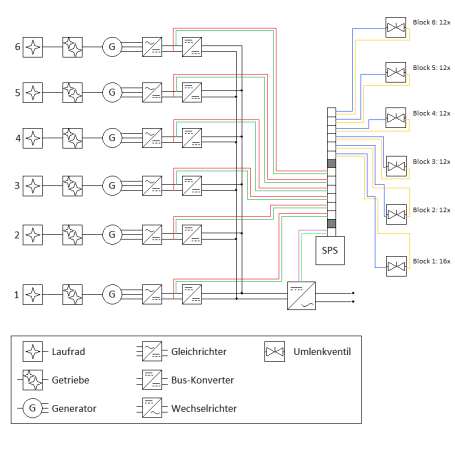
\includegraphics[width=14cm]{Skizze_GK4.png}
\caption{Prinzipschema}
\label{fig:Prinzipschema}
\end{figure}

Die potentielle Energie des Abwassers wird über ein Laufrad in kinetische Energie umgewandelt. Mit einem Getriebe wird die vom Laufrad kommende Drehzahl dem Generator angepasst, welcher die kinetische Energie in elektrische umwandelt. Der Gleichrichter transformiert den Dreiphasenwechselstrom in einen zweipoligen Gleichstrom. Anschliessend wird durch ein DC-DC Konverter eine Rückkoppelung auf den Genreator verhindert. Weiter stellt der Konverter sicher, dass eine stabile Ausgangsspannung anliegt und der DC-Bus galvanisch von Generator und Wechselrichter getrennt ist. Die summierte Energie aller sechs Generatorenstränge wird über einen Wechselrichter ins Stromnetz eingespeist. Zur Überwachung und auch zur Ansteuerung der Umlenkventile wird eine SPS verwendet.

\bigskip

\paragraph{Generator} \label{para:generator}

Der Wasserverbrauch und somit die Abwasserproduktion im Hochhaus ist nicht über den ganzen Tag konstant. Für die Dimensionierung der Bauteile ist es aber wichtig, den Spitzenwert der Abwasserproduktion zu kennen. Dieser kann aus Abbildung \ref{fig:tagesGangKurve} ausgelesen werden und liegt zwischen 7 und 8 Uhr morgens. Während dieser Stunde fliesst etwa 15\% des Abwassers ab, also müssen alle Komponenten auf diese Spitzenbelastung ausgelegt sein. 
Der unterste Lift ist am längsten und befördert gleichzeitig die gesamte Abwassermenge. Es wurde berechnet, dass er pro Tag \(70.22 MJ\) potentielle Energie aufnimmt. Mit einem Wirkungsgrad von 80\% des Liftes ergibt das 56.3 MJ, die der Generator umsetzten muss, \(15\%\) oder \(8.4 MJ\) dieser Energie zwischen 7 und 8 Uhr morgens. Der Generator muss also eine Mindestleitung von \(8.4 MJ / 3600 s = 2333 W \) aufweisen. Da die Abwassermenge auch während dieser Stunde nicht ganz konstant ist und zeitweise höher sein könnte, sollte der Generator eine Mindestleitung von \(3 kW\) haben.

\begin{figure}[H]
\centering
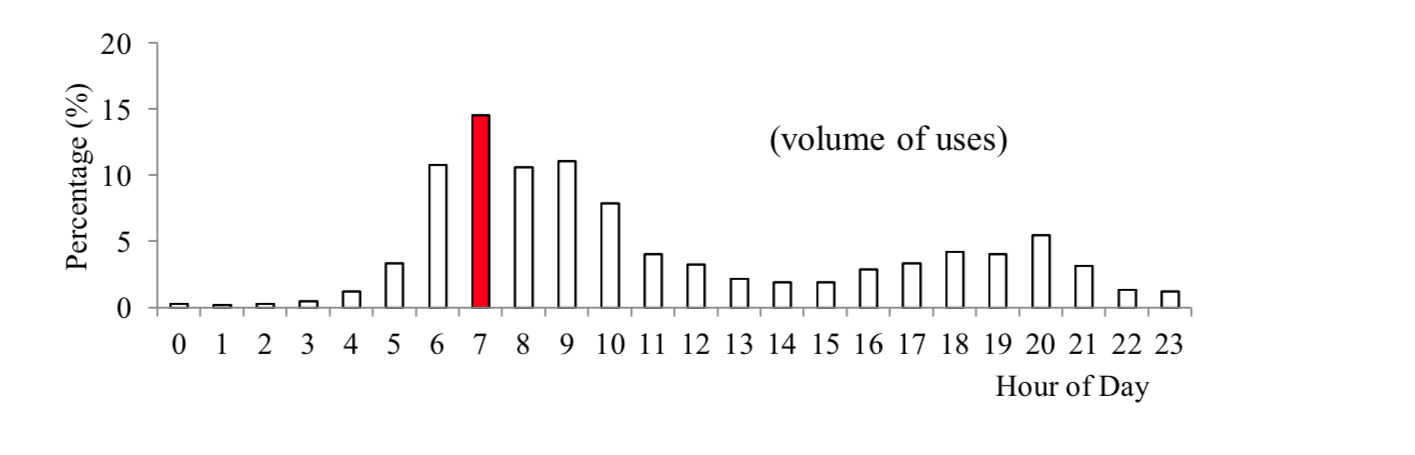
\includegraphics[width=\linewidth]{tagesGangKurve.png}
\caption{Typische Tagesgangkurve. \cite{peakWaterDemand}}
\label{fig:tagesGangKurve}
\end{figure}

Aufgrund dieser Berechnungen haben wir uns für einen Eastern Lion STC-3 Dreiphasengenerator entschieden (Siehe Abbildung \ref{fig:Generator}).  

\begin{figure}[H]
\centering
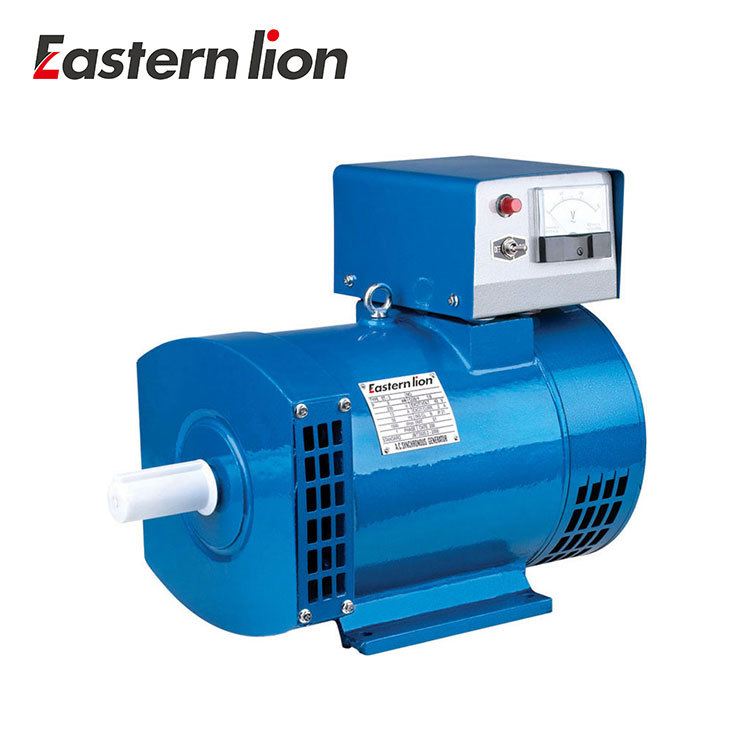
\includegraphics[width=6cm]{Generator.jpg}
\caption{Eastern Lion STC-3 \cite{generator}}
\label{fig:Generator}
\end{figure}

Dieser Generator ist mit einem Preis von 110\$ sehr günstig und erfüllt mit einer Leistung von 3 kW unsere Anforderungen.

\textbf{Leistung:}		3KW \newline
\textbf{Ausgang:}		3 Phasen 380V/120V \newline
\textbf{Drehzahl:}		1500 bis 1800 U/min \newline
\textbf{Wirkungsgrad:}	92\% \newline
\textbf{Kosten:}		110\$ \newline

\paragraph{Gleichrichtung nach Generator}

Die dreiphasige Wechselspannung des Generators wird mit einem Gleichrichter in Gleichspannung umgewandelt. Wir haben uns für einen SETEC SET4850 Gleichrichter entschieden (siehe Abbildung \ref{fig:Gleichrichter}). Dieser besteht nicht nur aus einem Dreiphasen-Gleichrichter, sondern ist auch ein Netzteil, das unter anderem einen geregelten \(48Vdc\) Ausgang hat. Dieser Ausgang kann somit direkt über den DC Bus mit den Wechselrichtern der anderen Turbinen parallel geschaltet werden. Gesteuert und überwacht wird das Gerät über einen RS 485 Bus.

\begin{figure}[H]
\centering
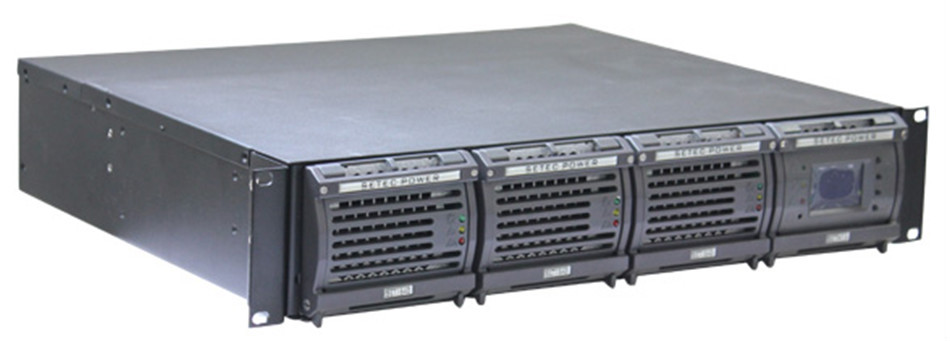
\includegraphics[width=6cm]{Gleichrichter.jpg}
\caption{Setec SET4850 \cite{gleichrichter}}
\label{fig:Gleichrichter}
\end{figure}

\textbf{Leistung:}		\(3 kW\) 			\newline
\textbf{Eingang:}		AC \(3 * 380V\) 	\newline
\textbf{Ausgang:}		DC 48V/110V/220V 	\newline
\textbf{Genauigkeit:}	\(\pm 0.5 \%\)		\newline
\textbf{Wirkungsgrad:}	\(96\%\) 			\newline
\textbf{Steuerung:}		RS 485 				\newline
\textbf{Kosten:}		300\$				\newline

%http://www.farnell.com/datasheets/2333819.pdf?_ga=2.222713307.1750103157.1543910091-374399726.1543659672

\paragraph{DC-DC Wandler}
Ein DC-DC Bus Konverter ist nicht nötig, da der SET4850 schon einen geregelten, galvanisch getrennten Ausgang hat. Dieser kann direkt auf den DC Bus geführt werden.

%TODO Paragraph entfernen?

\paragraph{Wechselrichter für Netzeinspeisung} \label{par:WechselrichterNetz}

Damit die gewonnen Leistung in das Netz eingespiesen werden kann, muss der Wechselrichter folgende Eigenschaften aufweisen. 

\textbf{Leistung:}		9KW \newline
\textbf{Ausgang:}		3Phasen \newline
\textbf{Kosten:}		Die Kosten sollen möglichst gering gehalten werden. \newline

In der Förderungsanlage wird ein Asynchrongenerator verbaut. Die Firma Voltacon ist bekannt für ihre Hochleistungswechselrichter.

Das Modell Hybrid Wechselrichter HSI10000 entspricht den gewünschten Anforderungen für unsere Förderungsanlage. Der Wechselrichter transformiert die 48VDC auf 230VAC mit einer Frequenz von 50\si{\hertz}. Das Gerät kann bis zu einer Leistung von 10KW erbringen. Mittels integrierten Displays kann die erbrachte Leistung zusätzlich abgelesen werden. 

Gemäss Datenblatt lassen sich Ströme bis 200A regeln. Der Wechselrichter hat einen netzunabhängigen Energiespeicher (Batterie-Backup). Um die Daten des Wechselrichters weiterzuleiten stehen verschieden Kommunikationsmittel zur Verfügung. Die Informationen können über einen USB Port, RS-232 oder den SNMP (Simple Network Management Protocol) Überwachungssoftware für Echtzeitstatusanzeige und -steuerung übermittelt werden. Die Kosten des Wechselrichters belaufen sich auf 3'401\si{Fr}.

\newpage


\paragraph{Kontrollsystem}

Das Kontrollsystem steuert und überwacht die Anlage und ist wie folgt aufgebaut: Auf einem PC ist eine C\# Software installiert. Das Programm kommuniziert über ModbusTPC mit der SPS und kann die Anlage so steuern. In der Abbildung \ref{fig:beckhoff} \nameref{fig:beckhoff} ist die SPS von Beckhoff ersichtlich.

\bigskip

\begin{figure} [H]
	\centering
	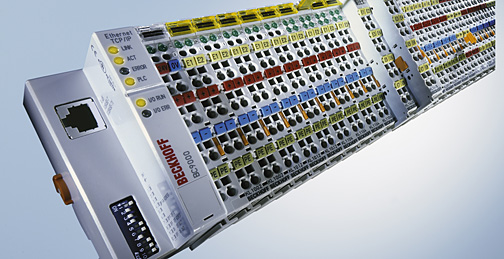
\includegraphics[width=10cm]{Beckhoff.jpg}
	\caption{SPS von Beckhoff \cite{beckhoff}}
	\label{fig:beckhoff}
\end{figure}

In der Software kann über eine grafische Oberfläche ein Benutzer einfach auf die Anlage zugreifen, steuern und Informationen ablesen. Das Programm hat zwei verschiedene Modi. Einen manuellen Modus und einen Betriebsmodus. Im manuellen Modus kann der Betrieb der Anlage für Wartungsarbeiten angepasst werden. So können die Ventile einzeln oder blockweise geschaltet werden. Im Betriebsmodus werden nur im Störungsfall die Ventile automatisch geschalten, um die Sicherheit zu gewährleisten. Wenn möglich werden nur einzelne Blöcke deaktiviert, damit die Anlage weiterhin Strom produzieren kann. In beiden Modi wird die Stromgewinnung überwacht. So wird angezeigt, welcher Generator gerade wie viel Strom erzeugt. Der Wechselrichter, der unter Wechselrichter für Netzeinspeisung beschrieben ist, kann über einem USB-Port eine serielle Kommunikation mit dem PC aufbauen. Das Programm kann die Informationen der aktuellen Energiegewinnung über diese Schnittstelle auslesen, speichert diese in einem Log. File und gibt diese an die Benutzeroberfläche weiter. Die gesammelten Daten können im Programm ausgewertet und grafisch dargestellt werden. Für dieses Kontrollsystem werden folgende Komponenten benötigt.

\bigskip

\begin{table}[H]
\small
\begin{tabular}{lllll}
\textbf{Anzahl}&\textbf {Komponente}&\textbf{Bezeichnung}&\textbf{Stückpreis [\si{CHF}]}&\textbf{Gesamtpreis [\si{CHF}]}\\
\hline
1&Kontrollklemme&BK9050&200&200\\
20&Digitale Ausgangsklemme&KL1114&100&2000\\
20&Digitale Eingangsklemme&KL2134&100&2000\\
7& Analoge Eingangsklemme&KL2134&100&700\\
1&PC&Dell&1000&1000\\
\hline
\end{tabular}
\end{table}

\bigskip

Die Kosten für die Komponenten betragen 5900 \si{Fr} \cite{beckhoff}. Für die Entwicklung der Software werden 3 PM benötigt, was einmalig 48'000\si{Fr} kostet. 



\newpage


\subsection{Mechanik}

\paragraph{Rohrkette}

In der Industrie werden Rohrkettenförderer für den Transport von Schuttgüter verwendet. In der Abbildung \ref{fig:Rohrkettenfoerderer} \nameref{fig:Rohrkettenfoerderer} ist der Innenaufbau eines solchen Rohrkettenförderers ersichtlich.

\begin{figure} [H]
	\centering
	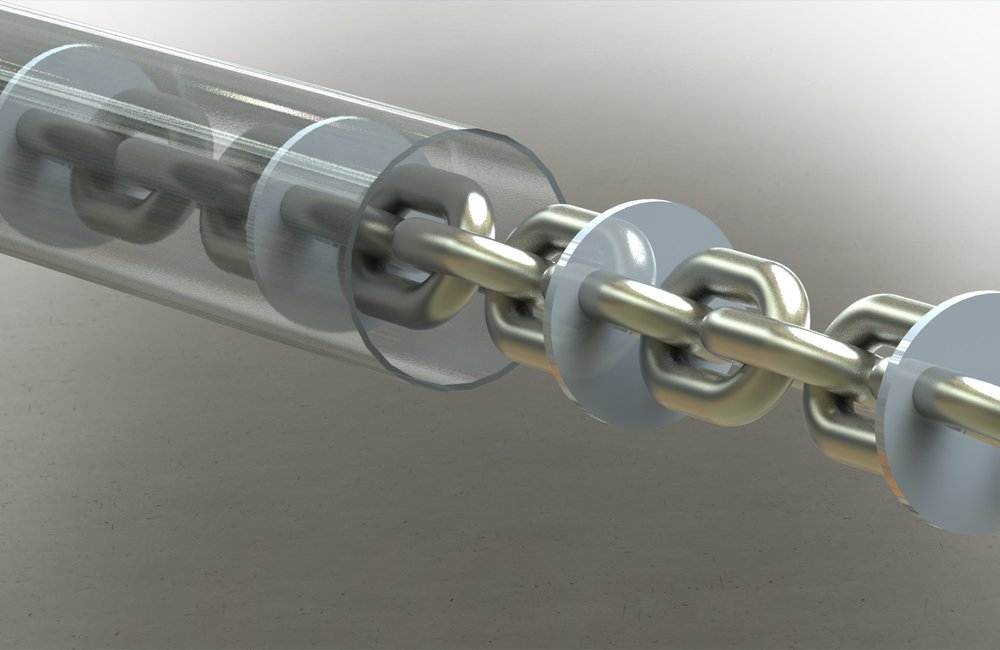
\includegraphics[width=6cm]{Rohrkettenfoerderer.jpg}
	\caption{Innenaufbau Rohrkettenförderer \cite{abconvey}}
	\label{fig:Rohrkettenfoerderer}
\end{figure}

Wir wollen keinen Schutt nach oben befördern, daher muss dieses System auf unsere Anforderungen angepasst werden. Diese Anforderungen sind, dass die verwendeten Materialien Robust gegenüber Korrosion sind, da das Abwasser aggressiv auf diese wirkt. Weiter müssen, um einen möglichst hohen Wirkungsgrad zu erreichen, die Platten mit möglichst kleinem Spielraum zur Aussenwand konstruiert werden, damit das Wasser nicht einfach auf der Seite herunterfliessen kann und gleichzeitig nicht eine zu grosse Reibung erzeugt wird. Die Drehachse, an dem der Generator angeschlossen wird, ist ein Stösselkettenrad. Dieses ist in der Abbildung \ref{fig:stoesselkettenrad} \nameref{fig:stoesselkettenrad} zu sehen

\begin{figure} [H]
	\centering
	\includegraphics[width=6cm]{Stoesselkettenrad.jpg}
	\caption{Stösselkettenrad \cite{schrage}}
	\label{fig:stoesselkettenrad}
\end{figure}


Um diesen Wasserlift zu bauen, beauftragen wir die Firma Schrage, ein führender Speziallist für Rohrketten, die in Deutschland zu Hause ist. Die Kosten belaufen sich für die 60.08\si{m} Höhendifferenz auf ca. 10'000\si{Fr} pro Lift und für die 80.24\si{m} Höhendifferenz auf ca. 13'000\si{Fr}. Insgesamt würde die Analage mit den Rohrketten, Rohr und Stösselkettenrad ca. 63'000\si{Fr} kosten. \cite{schrage}

\newpage

\paragraph{Zahnradsytem}
Da der Generator eine viel höhere Drehzahl benötigt, als dass der Lift zur Verfügung stellt, muss ein Getriebe verwendet werden. Doch um dieses zu dimensionieren, muss man zuerst wissen, wie schnell sich der Wasserlift überhaupt bewegt. Dies ist abhängig von der Wassermenge und vom Rohrdurchmesser. Das Modellhochhaus hat 76 bewohnte Stockwerke mit je fünf Bewohnern, die durchschnittlich 314 Liter Wasser am Tag verbrauchen. Die Gesamtwassermenge beträgt also \(76 * 5 * 314 = 119320 l/24h\), die vollständig durch den untersten Wasserlift abfliesst. Anhand der Tagesgangkurve (siehe Abbildung \ref{fig:tagesGangKurve}) kann man ablesen, dass 15\% des Abwassers zwischen 7 und 8 Uhr morgens abgelassen wird. Dies entspricht einer Abwassermenge von \(119320 * 0.15 = 17898 l\), etwa \(18 m^3 \), die innerhalb einer Stunde durch den untersten Wasserlift muss. Aus den Tabellen zu den Fördermengen von Schrage (Siehe Abbildung \ref{fig:foerdermengen}) kann man nun ablesen, bei welchem Rohrdurchmesser welche Geschwindigkeit nötig ist, um diese 18 Kubikmeter Abwasser zu befördern. 

\begin{figure} [H]
	\centering
	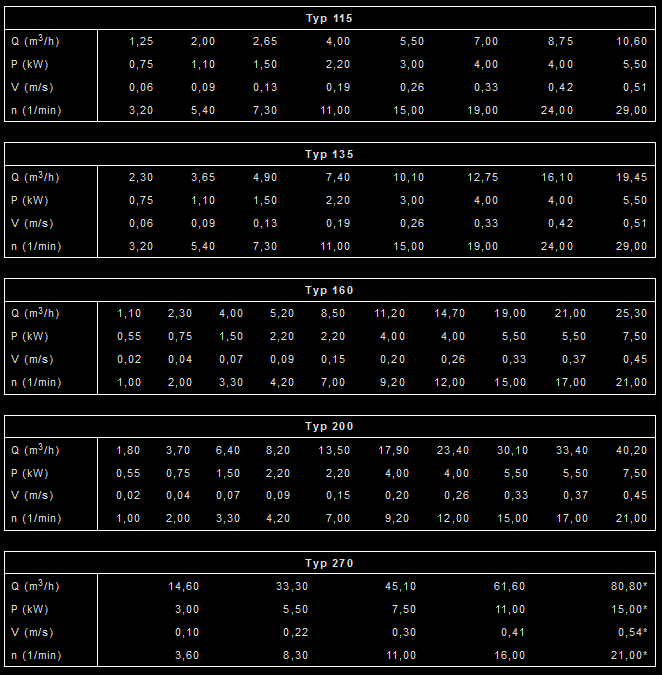
\includegraphics[width=12cm]{Foerdermengen.PNG}
	\caption{Fördermengen \cite{schrage}}
	\label{fig:foerdermengen}
\end{figure}

Um etwas Reserve zu haben, falls einmal eine grössere Abwasserspitze auftritt, sollte das Rohr einen Durchmesser von mindestens \(160mm\) haben. Bei \(18 m^3 /h \) und einem Rohrdurchmesser von \(160mm\) hat die Förderkette also eine Geschwindigkeit von etwa \(0.3 m/s \). Bei diesem Rohrdurchmesser hat das Stösselkettenrad einen Durchmesser von etwa \(400mm\)\cite{schrage} und einen Umfang von \(400mm * \pi = 1257mm = 1.257m\). Somit hat das Stösselkettenrad eine Drehzahl von \(1.257m * 0.3 m/s * 60s = 22,6 U/min\). Aufgrund der kleinen Drehzahl aber relativ grossen Leistung von maximal \(2300 W\) hat der Wasserlift ein relativ hohes Drehmoment von \( 2300 /(2 * \pi * 22.6/ 60) = 972 N/m\). Der Generator hat eine maximale Drehzahl von \(1800 U/min\), braucht aber nur wenig Drehmoment. Das Getriebe muss also die Drehzahl des Liftes erhöhen, dabei ist das nötige Übersetzungsverhältnis etwa 1:80. 
\textbf{Anforderungen an das Getriebe:}				\newline
\textbf{Übersetzungsverhältnis:}	1:80			\newline
\textbf{Leistung:}					\(>=3 kW\)		\newline
\textbf{Eingangsdrehzahl:}			\(22.6 U/min\)	\newline
\textbf{Eingangsdrehmoment:}		\(>=1000 Nm\)§	\newline
\textbf{Ausgangsdrehzahl:}			\(1800 U/min\)	\newline
\textbf{Ausgangsdrehmoment:}		\(>= 20 Nm\)	\newline

%TODO bin noch am Hersteller/Preis suchen.

\paragraph{Umleitventil}

Da wir für Störungsfälle eine Fallleitung eingeplant haben, muss ein Umleitungsventil installiert werden. Das Modell F7125 3-Way Butterfly Valve ist optimal für diese Bedingung geeignet. Das zugehörige Steuerungsmodell PRBUP-3-T kann von einer Spannung zwischen 24V-230V angesteuert werden. Somit können wir es im SPS System integrieren. Das Umleitungsventil hat ein Gesamtgewicht von 51\si{kg}. Für das ganze System kommt man auf Kosten von 2082\si{Fr}.

 \begin{figure} [H]
	\centering
	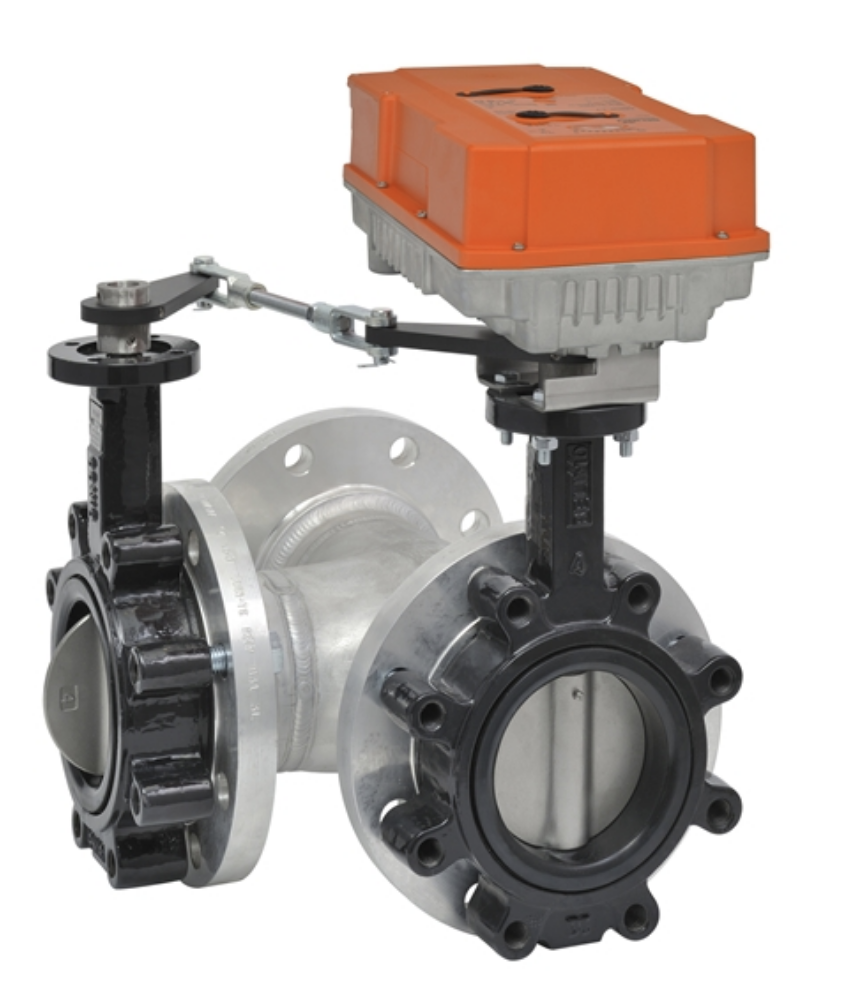
\includegraphics[width=6cm]{Umleitungsventil.png}
	\label{fig:Umleitungsventil}
\end{figure}


\cite{Belimo}



\subsection{Kosten}

%TODO Frank: Alle Kosten zusammentragen